%==============================================================
%  Kabir Singh — Curriculum Vitae (Prehealth)
%  GENERATED from data/cv.json by tools/build.py. Edit the CV
%  through admin.html (or data/cv.json), not this file: it is
%  rewritten on every build. Layout and styles: preamble.tex.
%==============================================================
%==============================================================
%  Kabir Singh — CV layout and styles.
%  Every cv*.tex (generated from data/cv.json, one per profile)
%  starts with %==============================================================
%  Kabir Singh — CV layout and styles.
%  Every cv*.tex (generated from data/cv.json, one per profile)
%  starts with %==============================================================
%  Kabir Singh — CV layout and styles.
%  Every cv*.tex (generated from data/cv.json, one per profile)
%  starts with \input{preamble}. Change fonts, spacing and the
%  entry macros here; the .docx copies these choices by hand.
%==============================================================
\documentclass[11pt,a4paper]{article}

\usepackage[T1]{fontenc}
\usepackage[utf8]{inputenc}
\usepackage{charter}
\usepackage[margin=1.8cm,includefoot,footskip=0.8cm]{geometry}
\usepackage{xcolor,enumitem,array,tabularx,needspace,fancyhdr,lastpage,microtype,multicol,graphicx}
\usepackage[hidelinks]{hyperref}

\definecolor{promptgray}{gray}{0.46}
\setlength{\parindent}{0pt}
\setlength{\parskip}{0pt}
\setlist[itemize]{leftmargin=1.3em,topsep=1pt,itemsep=0pt,parsep=0pt,partopsep=0pt}
\setlength{\tabcolsep}{0pt}
\emergencystretch=2em
\pagestyle{fancy}\fancyhf{}
\renewcommand{\headrulewidth}{0pt}\renewcommand{\footrulewidth}{0pt}
\setlength{\headheight}{14pt}
\setlength{\multicolsep}{2pt}
\fancyfoot[R]{\footnotesize Page \thepage\ of \pageref{LastPage}}
% the left footer ("Kabir Singh · Curriculum Vitae · <as of>") is set in each cv*.tex

%---- Section headings: faux small caps + rule ------------------
% Charter BT has no small caps: each word keeps a full-size initial
% and the rest is uppercase at \footnotesize.
\makeatletter
\def\fauxsc#1{\@fsc#1 \@@}
\def\@fsc#1 #2\@@{\@fscw#1\@@\if\relax\detokenize{#2}\relax\else\ \@fsc#2\@@\fi}
\def\@fscw#1#2\@@{#1{\footnotesize\MakeUppercase{#2}}}
\makeatother
% each heading also adds a PDF bookmark (the outline in a viewer's sidebar); subheadings nest under it
\hypersetup{bookmarksopen=true}
\newcounter{cvmark}
\newcommand{\cvsection}[1]{\needspace{3\baselineskip}\vspace{9pt}\stepcounter{cvmark}\pdfbookmark[0]{#1}{cvmark.\thecvmark}{\fauxsc{#1}}\par\vspace{2pt}\hrule height .45pt\vspace{5pt}}
\newcommand{\subhead}[1]{\needspace{2\baselineskip}\vspace{4pt}\stepcounter{cvmark}\pdfbookmark[1]{#1}{cvmark.\thecvmark}{\itshape #1}\par\vspace{2pt}}

%---- Entries ----------------------------------------------------
% One gap before every entry; tune it to change the density.
\newlength{\entrygap}\setlength{\entrygap}{4pt}
% \headentry{title}{dates}{second line}{right of second line}
%   two lines: bold title + dates, then organisation + (second date line, location)
\newcommand{\headentry}[4]{\needspace{2\baselineskip}\vspace{\entrygap}\noindent\begin{tabularx}{\linewidth}{@{}X@{\hspace{1em}}r@{}}\textbf{#1}&#2\\[-1pt]#3&#4\end{tabularx}\par}
% \lineentry{text}{dates}: one line, as in the two-page CV
\newcommand{\lineentry}[2]{\needspace{1.3\baselineskip}\vspace{\entrygap}\noindent\begin{tabularx}{\linewidth}{@{}>{\raggedright\arraybackslash}X@{\hspace{1em}}r@{}}#1 & #2\end{tabularx}\par}
% \roleline{text}{dates}: one of several roles under an entry (no gap above)
\newcommand{\roleline}[2]{\noindent\begin{tabularx}{\linewidth}{@{}>{\raggedright\arraybackslash}X@{\hspace{1em}}r@{}}#1 & #2\end{tabularx}\par}
% \project{title}: an italic project title under a research position
\newcommand{\project}[1]{\needspace{2\baselineskip}\vspace{1pt}\noindent{\itshape #1}\par}
% grey note to self, printed only by profiles with prompts on
\newcommand{\prompt}[1]{\begin{itemize}[leftmargin=1.45em]\item[\textcolor{promptgray}{$\rightarrow$}]\textcolor{promptgray}{\itshape #1}\end{itemize}}
% label / text rows (coursework, skills)
\newcommand{\course}[2]{\noindent\begin{tabularx}{\linewidth}{@{}>{\itshape}p{3.3cm}@{\hspace{0.5em}}X@{}}#1 & #2\end{tabularx}\par}
% presentations: citation, then one row per venue
\newcommand{\pres}[1]{\needspace{4\baselineskip}\vspace{\entrygap}\noindent #1\par}
\newcommand{\venue}[3]{\noindent\hspace*{1.0em}\begin{tabularx}{\dimexpr\linewidth-1em\relax}{@{}X@{\hspace{1em}}r@{}}#1 (\emph{#2}) & #3\end{tabularx}\par}
. Change fonts, spacing and the
%  entry macros here; the .docx copies these choices by hand.
%==============================================================
\documentclass[11pt,a4paper]{article}

\usepackage[T1]{fontenc}
\usepackage[utf8]{inputenc}
\usepackage{charter}
\usepackage[margin=1.8cm,includefoot,footskip=0.8cm]{geometry}
\usepackage{xcolor,enumitem,array,tabularx,needspace,fancyhdr,lastpage,microtype,multicol,graphicx}
\usepackage[hidelinks]{hyperref}

\definecolor{promptgray}{gray}{0.46}
\setlength{\parindent}{0pt}
\setlength{\parskip}{0pt}
\setlist[itemize]{leftmargin=1.3em,topsep=1pt,itemsep=0pt,parsep=0pt,partopsep=0pt}
\setlength{\tabcolsep}{0pt}
\emergencystretch=2em
\pagestyle{fancy}\fancyhf{}
\renewcommand{\headrulewidth}{0pt}\renewcommand{\footrulewidth}{0pt}
\setlength{\headheight}{14pt}
\setlength{\multicolsep}{2pt}
\fancyfoot[R]{\footnotesize Page \thepage\ of \pageref{LastPage}}
% the left footer ("Kabir Singh · Curriculum Vitae · <as of>") is set in each cv*.tex

%---- Section headings: faux small caps + rule ------------------
% Charter BT has no small caps: each word keeps a full-size initial
% and the rest is uppercase at \footnotesize.
\makeatletter
\def\fauxsc#1{\@fsc#1 \@@}
\def\@fsc#1 #2\@@{\@fscw#1\@@\if\relax\detokenize{#2}\relax\else\ \@fsc#2\@@\fi}
\def\@fscw#1#2\@@{#1{\footnotesize\MakeUppercase{#2}}}
\makeatother
% each heading also adds a PDF bookmark (the outline in a viewer's sidebar); subheadings nest under it
\hypersetup{bookmarksopen=true}
\newcounter{cvmark}
\newcommand{\cvsection}[1]{\needspace{3\baselineskip}\vspace{9pt}\stepcounter{cvmark}\pdfbookmark[0]{#1}{cvmark.\thecvmark}{\fauxsc{#1}}\par\vspace{2pt}\hrule height .45pt\vspace{5pt}}
\newcommand{\subhead}[1]{\needspace{2\baselineskip}\vspace{4pt}\stepcounter{cvmark}\pdfbookmark[1]{#1}{cvmark.\thecvmark}{\itshape #1}\par\vspace{2pt}}

%---- Entries ----------------------------------------------------
% One gap before every entry; tune it to change the density.
\newlength{\entrygap}\setlength{\entrygap}{4pt}
% \headentry{title}{dates}{second line}{right of second line}
%   two lines: bold title + dates, then organisation + (second date line, location)
\newcommand{\headentry}[4]{\needspace{2\baselineskip}\vspace{\entrygap}\noindent\begin{tabularx}{\linewidth}{@{}X@{\hspace{1em}}r@{}}\textbf{#1}&#2\\[-1pt]#3&#4\end{tabularx}\par}
% \lineentry{text}{dates}: one line, as in the two-page CV
\newcommand{\lineentry}[2]{\needspace{1.3\baselineskip}\vspace{\entrygap}\noindent\begin{tabularx}{\linewidth}{@{}>{\raggedright\arraybackslash}X@{\hspace{1em}}r@{}}#1 & #2\end{tabularx}\par}
% \roleline{text}{dates}: one of several roles under an entry (no gap above)
\newcommand{\roleline}[2]{\noindent\begin{tabularx}{\linewidth}{@{}>{\raggedright\arraybackslash}X@{\hspace{1em}}r@{}}#1 & #2\end{tabularx}\par}
% \project{title}: an italic project title under a research position
\newcommand{\project}[1]{\needspace{2\baselineskip}\vspace{1pt}\noindent{\itshape #1}\par}
% grey note to self, printed only by profiles with prompts on
\newcommand{\prompt}[1]{\begin{itemize}[leftmargin=1.45em]\item[\textcolor{promptgray}{$\rightarrow$}]\textcolor{promptgray}{\itshape #1}\end{itemize}}
% label / text rows (coursework, skills)
\newcommand{\course}[2]{\noindent\begin{tabularx}{\linewidth}{@{}>{\itshape}p{3.3cm}@{\hspace{0.5em}}X@{}}#1 & #2\end{tabularx}\par}
% presentations: citation, then one row per venue
\newcommand{\pres}[1]{\needspace{4\baselineskip}\vspace{\entrygap}\noindent #1\par}
\newcommand{\venue}[3]{\noindent\hspace*{1.0em}\begin{tabularx}{\dimexpr\linewidth-1em\relax}{@{}X@{\hspace{1em}}r@{}}#1 (\emph{#2}) & #3\end{tabularx}\par}
. Change fonts, spacing and the
%  entry macros here; the .docx copies these choices by hand.
%==============================================================
\documentclass[11pt,a4paper]{article}

\usepackage[T1]{fontenc}
\usepackage[utf8]{inputenc}
\usepackage{charter}
\usepackage[margin=1.8cm,includefoot,footskip=0.8cm]{geometry}
\usepackage{xcolor,enumitem,array,tabularx,needspace,fancyhdr,lastpage,microtype,multicol,graphicx}
\usepackage[hidelinks]{hyperref}

\definecolor{promptgray}{gray}{0.46}
\setlength{\parindent}{0pt}
\setlength{\parskip}{0pt}
\setlist[itemize]{leftmargin=1.3em,topsep=1pt,itemsep=0pt,parsep=0pt,partopsep=0pt}
\setlength{\tabcolsep}{0pt}
\emergencystretch=2em
\pagestyle{fancy}\fancyhf{}
\renewcommand{\headrulewidth}{0pt}\renewcommand{\footrulewidth}{0pt}
\setlength{\headheight}{14pt}
\setlength{\multicolsep}{2pt}
\fancyfoot[R]{\footnotesize Page \thepage\ of \pageref{LastPage}}
% the left footer ("Kabir Singh · Curriculum Vitae · <as of>") is set in each cv*.tex

%---- Section headings: faux small caps + rule ------------------
% Charter BT has no small caps: each word keeps a full-size initial
% and the rest is uppercase at \footnotesize.
\makeatletter
\def\fauxsc#1{\@fsc#1 \@@}
\def\@fsc#1 #2\@@{\@fscw#1\@@\if\relax\detokenize{#2}\relax\else\ \@fsc#2\@@\fi}
\def\@fscw#1#2\@@{#1{\footnotesize\MakeUppercase{#2}}}
\makeatother
% each heading also adds a PDF bookmark (the outline in a viewer's sidebar); subheadings nest under it
\hypersetup{bookmarksopen=true}
\newcounter{cvmark}
\newcommand{\cvsection}[1]{\needspace{3\baselineskip}\vspace{9pt}\stepcounter{cvmark}\pdfbookmark[0]{#1}{cvmark.\thecvmark}{\fauxsc{#1}}\par\vspace{2pt}\hrule height .45pt\vspace{5pt}}
\newcommand{\subhead}[1]{\needspace{2\baselineskip}\vspace{4pt}\stepcounter{cvmark}\pdfbookmark[1]{#1}{cvmark.\thecvmark}{\itshape #1}\par\vspace{2pt}}

%---- Entries ----------------------------------------------------
% One gap before every entry; tune it to change the density.
\newlength{\entrygap}\setlength{\entrygap}{4pt}
% \headentry{title}{dates}{second line}{right of second line}
%   two lines: bold title + dates, then organisation + (second date line, location)
\newcommand{\headentry}[4]{\needspace{2\baselineskip}\vspace{\entrygap}\noindent\begin{tabularx}{\linewidth}{@{}X@{\hspace{1em}}r@{}}\textbf{#1}&#2\\[-1pt]#3&#4\end{tabularx}\par}
% \lineentry{text}{dates}: one line, as in the two-page CV
\newcommand{\lineentry}[2]{\needspace{1.3\baselineskip}\vspace{\entrygap}\noindent\begin{tabularx}{\linewidth}{@{}>{\raggedright\arraybackslash}X@{\hspace{1em}}r@{}}#1 & #2\end{tabularx}\par}
% \roleline{text}{dates}: one of several roles under an entry (no gap above)
\newcommand{\roleline}[2]{\noindent\begin{tabularx}{\linewidth}{@{}>{\raggedright\arraybackslash}X@{\hspace{1em}}r@{}}#1 & #2\end{tabularx}\par}
% \project{title}: an italic project title under a research position
\newcommand{\project}[1]{\needspace{2\baselineskip}\vspace{1pt}\noindent{\itshape #1}\par}
% grey note to self, printed only by profiles with prompts on
\newcommand{\prompt}[1]{\begin{itemize}[leftmargin=1.45em]\item[\textcolor{promptgray}{$\rightarrow$}]\textcolor{promptgray}{\itshape #1}\end{itemize}}
% label / text rows (coursework, skills)
\newcommand{\course}[2]{\noindent\begin{tabularx}{\linewidth}{@{}>{\itshape}p{3.3cm}@{\hspace{0.5em}}X@{}}#1 & #2\end{tabularx}\par}
% presentations: citation, then one row per venue
\newcommand{\pres}[1]{\needspace{4\baselineskip}\vspace{\entrygap}\noindent #1\par}
\newcommand{\venue}[3]{\noindent\hspace*{1.0em}\begin{tabularx}{\dimexpr\linewidth-1em\relax}{@{}X@{\hspace{1em}}r@{}}#1 (\emph{#2}) & #3\end{tabularx}\par}

\hypersetup{pdftitle={Kabir Singh -- Curriculum Vitae},pdfauthor={Kabir Singh}}
\fancyfoot[L]{\footnotesize Kabir Singh $\cdot$ Curriculum Vitae $\cdot$ October 2026}

\begin{document}
\noindent\begin{tabularx}{\linewidth}{@{}m{2.3cm}@{\hspace{1.1em}}>{\raggedright\arraybackslash}X@{}}
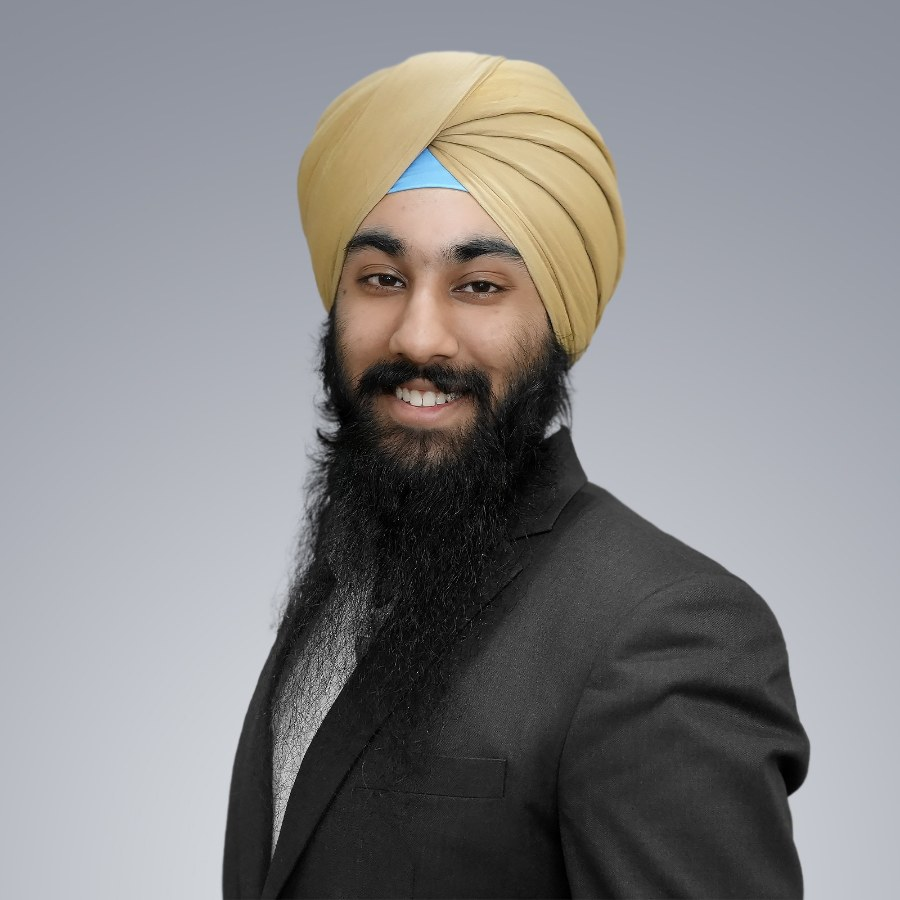
\includegraphics[width=2.3cm]{../images/cv/headshot-bqbvw8.jpg} & {\Large\bfseries Kabir Singh}\par\vspace{3pt}{\small \href{mailto:kabirsinghji@gmail.com}{kabirsinghji@gmail.com} $\cdot$
 +1 917 636 8664 $\cdot$
 \href{https://kabirsinghji.github.io}{kabirsinghji.github.io} $\cdot$
 \href{https://orcid.org/0009-0002-5159-5879}{ORCID 0009-0002-5159-5879}}
\end{tabularx}\par\vspace{-2pt}

\cvsection{Education}
\headentry{B.S. Mathematical Sciences (Mathematical Biology)}{Sep 2023 -- May 2027}{Albert Dorman Honors College \& Jordan Hu College of Sciences \& Liberal Arts, NJIT}{\begin{tabular}[t]{@{}r@{}}(Expected)\\Newark, NJ, USA\end{tabular}}
\begin{itemize}
  \item Dean's List all semesters.
  \item Minors: \textbf{Biomedical Engineering Technology}, History, Philosophy \& Applied Ethics; Honors tracks: Medical Humanities \& Global Studies (first Honors College student to pursue two).
  \item Academic scholarships exceeding \$100,000, including Academic Excellence, Honors Merit, Honors Residential, \& Highlander Achievement scholarships; tuition \& board scholarship support.
\end{itemize}
\vspace{3pt}
\course{Biomedical}{\textbf{Applications in Healthcare}; Biochemistry; Biomedical Mechatronics; Cell \& Molecular Biology}
\course{Medicine \& society}{\textbf{Biomedical Ethics}; Health, Justice, \& Capitalism; Medical Sociology; \textbf{Medicine \& Law in Modern History}}
\course{Quantitative}{Applied Numerical Methods; Differential Equations (ordinary \& partial); \textbf{Linear Algebra}; \textbf{Mathematical Modeling}; Stochastic \& Discrete Models in Biology}
\course{Independent study}{Bioengineering (Dr Vivek Kumar); Maths (Dr James Maclaurin, Dr Horacio Rotstein); History (Dr Stephen Pemberton, Satnam Singh)}
\headentry{Exchange semester (Global E3), Lund University, Sweden}{Jan 2025 -- Jun 2025}{Faculty of Engineering (LTH); 44 ECTS}{Lund, Sweden}
\begin{itemize}
  \item Fellow, Institute of International Education's Global Engineering Education Exchange (Global E3).
\end{itemize}
\vspace{3pt}
\course{Master's level}{Biomathematics; Immunotechnology; Microscopy, Bio-Imaging; \textbf{Ultrasound Physics \& Technology}}
\course{Undergraduate}{Patent \& Intellectual Property Rights}

\cvsection{Research Experience}
\subhead{Computational \& Mathematical Biology}
\headentry{Undergraduate Researcher \& Computational Biology Team Lead}{Oct 2023 -- Present}{KumarLab; PI: Dr Vivek Kumar, University of Houston (previously NJIT)}{Houston, TX / Newark, NJ, USA}
\begin{itemize}
  \item Lead undergraduates \& graduates in computational development of peptide therapeutics; trained 15+ lab associates \& secured over \$15,000 in direct project funding.
  \item Conducted dissections \& assisted animal work on angiogenic hydrogels subsequently published; maintained computational research after the lab relocated to Houston.
\end{itemize}
\project{A novel cyclic peptide that blocks human autoimmune antibodies for the treatment of multiple sclerosis.}
\begin{itemize}
  \item Designed cyclic peptides against multiple sclerosis autoantibodies with eight-residue design scaffold \& Rosetta/FlexPepDock workflow; ran molecular-dynamics simulations for my top-ranked peptide CAP8, with GROMACS simulations \& alanine scanning; in the published study, CAP8 bound anti-GlialCAM autoantibody with \textit{K}\textsubscript{d} = 0.294 mM, versus 4.82 mM linear \& 2.61 mM unrelated cyclic controls \& cut epitope detection on Western blot by 69\% versus 27\% \& 5\% for controls.
  \item Partial work through `independent study' module, published in the \textit{European Journal of Medicinal Chemistry} [1].
\end{itemize}
\project{A novel cyclic peptide that blocks fertilization protein for a male contraceptive.}
\begin{itemize}
  \item Secured \& led a funded non-hormonal male-contraception project: machine-learning-guided cyclic peptide design against \textit{redacted target}, docking \& refinement.
  \item 8 poster presentations, scientific manuscript \& patent application in preparation [2].
\end{itemize}
\project{Lipidated self-assembled peptides that modulate GPCR signaling of CB1 receptor.}
\begin{itemize}
  \item Helped run in-silico validation using NAMD, GROMACS for membrane simulations, aggregation propensity, docking, \& persistence studies of peptide.
  \item Project still underway, simulations in progress, 1 poster presentation.
\end{itemize}
\headentry{Undergraduate Researcher, Computational Bionanotechnology}{Jun 2026 -- Present}{SoftNanoLab; PI: Prof Stefano Angioletti-Uberti, Imperial College London}{London, UK}
\project{Binder squeeze: mimicking natural binders.}
\begin{itemize}
  \item Apply statistical mechanics, molecular dynamics, protein language models \& machine-learning methods to enzyme \& binder design \& soft-matter/biomaterial systems; specifically developing methodology from previous papers ``Mind the Gap'' \& ``Squeezing Enzymes'' (preprint) to develop more efficient miniproteins derived from natural binders.
  \item Project still underway, contributed code to BAGEL (Biomolecular Algorithm for Guidance in Energy Landscape); investigate peptide designs that mimic natural ligands; develop mathematical theory \& equations from `squeeze' \& its complement `grow'.
\end{itemize}
\headentry{Undergraduate Researcher, Mathematical Oncology}{Sep 2026 -- Present}{PI: Dr Horacio Rotstein, NJIT}{Newark, NJ, USA}
\project{A simplified model of the MAPK/ERK pathway for therapeutic modeling.}
\begin{itemize}
  \item Derive reduced mathematical descriptions \& characterize retained dynamical properties for practical implementation.
  \item `Independent study' module, project still underway, poster in preparation.
\end{itemize}
\headentry{Undergraduate Researcher, Mathematical Modeling}{Oct 2025 -- May 2026}{PI: Dr James Maclaurin, NJIT}{Newark, NJ, USA}
\project{Modeling amyloid as an epidemic.}
\begin{itemize}
  \item Applied Hawkes self-exciting point processes in reframing A\ensuremath{\beta}42 secondary nucleation dynamics \& feedback in amyloid formation.
  \item `Independent study' module, project complete, internal paper for course written.
\end{itemize}
\subhead{Intellectual \& Cultural History}
\headentry{Emerging Scholars Research Fellow, Early Modern Sikh History}{Sep 2026 -- Dec 2026}{Harvard Sikh Center; mentor: Satnam Singh}{Remote}
\project{Dissemination and the making of Khalsa authority in a contested panth.}
\begin{itemize}
  \item How the early Khalsa came to dominate the wider Sikh world against rival claimants, including the Bandai Khalsa, Minas, Ram Raiyas \& Hindaliyas.
  \item Argue that the answer lies less in politics than in transmission: the Khalsa's consolidation of `authentic Sikh teachings' through \textit{katha} preceded \& enabled its control of the panth.
  \item Sources: Gurmukhi \& Persian primary materials, including works attributed to Bhai Mani Singh, \textit{hukamname}, \textit{rahit-nama} \& sampardaic literature, alongside Persian \& European accounts of the period.
  \item Twelve-week fellowship term producing a paper \& a presentation: first, a characterization of the intellectual landscape \& its conflicts; second, a prosopography linking intellectual influences to the period's political figures.
\end{itemize}
\headentry{Undergraduate Researcher, History of Medicine \& Bioethics}{Sep 2026 -- Present}{PI: Dr Stephen Pemberton, NJIT}{Newark, NJ, USA}
\project{Physician, heal thyself: hidden death in American medicine.}
\begin{itemize}
  \item Trace the legal history of end-of-life decision-making from \textit{In re Quinlan} (1976) to \textit{Cruzan v. Director, Missouri Department of Health} (1990).
  \item Compare how three physician-authors, Sherwin Nuland, Atul Gawande \& Haider Warraich, account for dying in modern American medicine.
  \item `Independent study' module, project complete, academic manuscript in preparation.
\end{itemize}
\headentry{Undergraduate Researcher, Digital History \& Urban Studies}{Jan 2024 -- May 2024,}{PI: Dr Louis Hamilton, NJIT; field research in Rome \& Florence}{\begin{tabular}[t]{@{}r@{}}Jan 2026 -- May 2026\\Newark, NJ, USA / Italy\end{tabular}}
\begin{itemize}
  \item Two solo-authored geospatial narratives (StoryMapJS) mapping sites visited on foot against historical \& archival sources.
\end{itemize}
\project{Power vs.\ the People: the Via Giulia, Rome.}
\begin{itemize}
  \item Mapped 18 sites, layering Counter-Reformation Marian shrines against Julius II's 1508 papal axis along the Via Giulia, Rome, drawing on the Early Modern Rome Reconstructed database \& Rufini's 1853 shrine census; argued the street shows superimposition \& negotiation rather than a papal-versus-popular divide.
  \item Course project (HIST 328), complete; published online as a StoryMap.
\end{itemize}
\project{Processions and Power: Florence.}
\begin{itemize}
  \item Mapped 22 Florentine sites to examine how urban expansion transformed liturgical processions into contests of ecclesiastical \& household prestige, read against Dante's critique of the \textit{gente nuova}.
  \item Course project (HIST 329), complete; published online as a StoryMap.
\end{itemize}
\subhead{Emergency Care \& Health Services}
\headentry{Undergraduate Researcher, Collegiate Emergency Medical Services}{Sep 2025 -- Present}{PI: Dr Chang Yaramothu, NJIT}{Newark, NJ, USA}
\project{A comprehensive study of operational models in university based EMS organisations.}
\begin{itemize}
  \item Co-developed IRB protocol, questionnaire \& recruitment materials for a national study of collegiate EMS organizations; examined resources, organizational structures, operating models \& capabilities across US collegiate EMS squads.
  \item Data collection \& analysis underway.
\end{itemize}

\cvsection{Publications \& Manuscripts}
\begin{enumerate}[label={[\arabic*]},leftmargin=2.2em,itemsep=3pt,topsep=1pt,start=1]
  \item C.~Heffernan, O.~West, \textbf{K.~Singh}, J.~Dodd-o, M.~James, A.~Baradi, K.~Rybak, A.~Lateef, S.~Elkabes, V.~Kumar. ``A novel cyclic peptide that blocks human autoimmune antibodies for the treatment of multiple sclerosis.'' \textit{Eur. J.~Med. Chem.} (2026). \href{https://doi.org/10.1016/j.ejmech.2026.119173}{doi:10.1016/j.ejmech.2026.119173}\\
  \textit{Contribution:} ran the molecular dynamics simulations; designed the published peptide
  \item \textbf{K.~Singh}, C.~Heffernan, O.~West, J.~Dodd-o, V.~Kumar. ``Machine learning for rational design of a cyclic peptide-based male contraceptive.'' In preparation; patent application in preparation
  \item J.~Lau, D.~Yun, \textbf{K.~Singh}, A.~Patananan, N.~Jadavji. ``Academic publishing as a launchpad: how publishing research in an undergraduate journal shapes future careers.'' In preparation
\end{enumerate}

\cvsection{Presentations}
\pres{M.~Kotta, G.~Victorio, G.~Karmacharya, \textbf{K.~Singh}, N.~Giovannetti, B.~Shadpoor, J.~Dodd-O, V.~Kumar. ``Putative computational design of novel inhibitors to modulate de-novo targets for CB1 receptor.''}
\venue{University of Houston, Undergraduate Research Day}{Poster \& podium}{2026}
\pres{\textbf{K.~Singh}, C.~Heffernan, J.~Dodd-O, V.~Kumar. ``Development of a novel male contraceptive using cyclic peptides to inhibit fertilization.''}
\venue{AAP/ASCI/APSA Joint Meeting}{Poster}{2026}
\venue{NJIT AI Exploration Day}{Poster}{2026}
\venue{NJIT Honors Interdisciplinary Research Forum, first place}{Poster}{Fall 2025}
\venue{National Contraception Meeting}{Poster}{2025}
\venue{NJIT Honors Interdisciplinary Research Forum}{Poster}{Spring 2025}
\venue{NJIT Dana Knox Research Showcase}{Poster}{2025}
\venue{NJIT Undergraduate Research \& Innovation}{Abstract \& podium}{2025}
\venue{Biomedical Engineering Society (BMES), co-presenter}{Abstract \& poster}{2024}
\venue{NJIT Undergraduate Research \& Innovation}{Abstract \& podium}{2024}
\pres{\textbf{K.~Singh}, J.~Lau, H.~Gerber, A.~Alibilli, L.~Goralsky. ``Mitigating knowledge drain: a case study in optimizing workflow and training in a high-turnover, international peer-reviewed undergraduate science academic journal.''}
\venue{National Conference on Undergraduate Research (NCUR)}{Poster}{2026}

\cvsection{Lectures \& Features}
\lineentry{\textbf{Invited speaker (forthcoming), Science National Honor Society} -- Piscataway High School}{2026}
\lineentry{\textbf{\href{https://news.njit.edu/njit-students-meet-state-secretary-higher-education}{Invited student roundtable speaker}}}{2026}
\begin{itemize}
  \item Margo Chaly, New Jersey Secretary of Education; NJIT
\end{itemize}
\lineentry{\textbf{Invited speaker, NJIT University Advancement Dinner}}{2026}
\begin{itemize}
  \item Interdisciplinary medicine \& healthcare research for NJIT leadership, including interim president \& interim provost
\end{itemize}
\lineentry{\textbf{Speaker, `Shaping the Future of Healthcare \& Innovation' dinner}}{Oct 2026}
\begin{itemize}
  \item Peptide therapeutics, published multiple sclerosis research, \& emergency care; alongside Dr Genoa R.~Warner \& Dr Bryan Pfister, NJIT
\end{itemize}
\lineentry{\textbf{Lecture series, Ethics in Science and Research} -- Science Mentorship Institute}{2026}
\lineentry{\textbf{Session moderator, Student Oral Presentations (Communications)} -- NCUR}{2026}
\lineentry{\textbf{Featured presenter, `Navigating peer review and the student journal landscape'}}{2026}
\begin{itemize}
  \item `Shaping Asia's Future: Development, Innovation, and Society in Transition', Nazarbayev University / Asian Universities Alliance
\end{itemize}
\lineentry{\textbf{Featured panelist, `It's Different for Girls'}}{2026}
\begin{itemize}
  \item Documentary screening \& panel; NJIT ADHC \& CSLA co-sponsored colloquium
\end{itemize}
\lineentry{\textbf{NJIT Makes: Undergraduate Research and Innovation} -- NJIT promotional material}{2026}
\lineentry{\textbf{Invited speaker, NJIT Board of Trustees and President's Town Hall}}{2025}
\begin{itemize}
  \item Presented with NJIT First Aid Squad leadership at the request of President Teik Lim
\end{itemize}
\lineentry{\textbf{Honors in Action 2025}}{2025}
\begin{itemize}
  \item Albert Dorman Honors College publication: research, awards \& study abroad
\end{itemize}
\lineentry{\textbf{\href{https://news.njit.edu/150-honors-scholars-showcase-findings-interdisciplinary-research-forum}{Article feature: `150+ Honors Scholars Showcase Findings at Interdisciplinary Research Forum'}} -- Nayib Morán, NJIT News}{2025}
\lineentry{\textbf{Featured speaker, ADHC Advising Day} -- NJIT; appearances in both 2024 \& 2025}{2024, 2025}
\lineentry{\textbf{Honors in Action 2024}}{2024}
\begin{itemize}
  \item Albert Dorman Honors College publication: research \& study abroad
\end{itemize}
\lineentry{\textbf{\href{https://njitvector.com/19044/features/undergraduate-student-researchers-on-campus/}{Article feature: `Undergraduate Student Researchers on Campus'}}}{2024}
\begin{itemize}
  \item Gurnoor Kaur, \textit{The Vector}, NJIT student newspaper
\end{itemize}
\lineentry{\textbf{Lecture, `Introduction to PyMOL and Linear Peptide Design'} -- NJIT, Genetically Engineered Machines}{2024}

\cvsection{Research Funding \& Honours}
\subhead{Grants \& awards}
\lineentry{\textbf{Undergraduate Research Opportunities Programme (UROP) bursary}; \textasciitilde{}£100}{Jun -- Jul 2026}
\begin{itemize}
  \item Imperial College London, Department of Materials; project: using protein language models to mimic natural ligands
  \item Personal compensation included
\end{itemize}
\lineentry{\textbf{NSF I-Corps Regional Program, Northeast Hub}; \$750}{May -- Jun 2026}
\begin{itemize}
  \item Competitive cohort \& customer-discovery project funding for Axioma Therapeutics
\end{itemize}
\lineentry{\textbf{Grace Hopper AI Research Institute grant}; \$3,330}{May -- Aug 2025}
\begin{itemize}
  \item NJIT, computational protein design course development
\end{itemize}
\lineentry{\textbf{Honors College Moonshot Grant for Engaged Scholarship}; \$6,500; 1 recipient per annum}{Jun -- Jul 2025}
\begin{itemize}
  \item Male-contraceptive project
  \item Personal compensation included
\end{itemize}
\lineentry{\textbf{Male Contraceptive Initiative Youth Advisory Board project grant}; \$1,000; 1 recipient in 2025}{Jan -- Jun 2025}
\begin{itemize}
  \item Grantee-led male-contraceptive project
  \item Personal compensation included
\end{itemize}
\lineentry{\textbf{Male Contraceptive Initiative travel award}; \$500; only trainee selected}{May 2025}
\begin{itemize}
  \item National Contraception Meeting, Durham, North Carolina
\end{itemize}
\lineentry{\textbf{NJIT Undergraduate Research \& Innovation Student Seed Grant}; \$3,000}{Oct 2024 -- May 2025}
\begin{itemize}
  \item Phase-2 longitudinal research project, cyclic peptide therapeutic for multiple sclerosis
\end{itemize}
\lineentry{\textbf{Honors Summer Research Institute (HSRI) grant}; \$3,000}{Jun -- Jul 2024}
\begin{itemize}
  \item ADHC \& NJIT URI; multiple sclerosis \& male-contraceptive projects
  \item Personal compensation included
\end{itemize}
\lineentry{\textbf{First place, Honors Interdisciplinary Research Forum}}{Fall 2025}
\begin{itemize}
  \item Male-contraceptive poster, NJIT Albert Dorman Honors College
\end{itemize}
\lineentry{\textbf{Academic Excellence, Honors Merit, Honors Residential scholarships}}{2023 -- 2027}
\begin{itemize}
  \item NJIT merit scholarships, part of award package exceeding \$100,000
\end{itemize}
\lineentry{\textbf{Highlander Achievement Scholarship} -- NJIT}{2023 -- 2027}
\subhead{Fellowships \& selective programmes}
\lineentry{\textbf{Emerging Scholars Research Fellowship}}{2026}
\begin{itemize}
  \item Harvard Sikh Center; early modern Sikh history
\end{itemize}
\lineentry{\textbf{Honors Summer Research Institute Fellowship} -- Fellow}{\begin{tabular}[t]{@{}r@{}}Jun 2024 -- Jul 2024,\\Jun 2025 -- Jul 2025\end{tabular}}
\lineentry{\textbf{Goldwater Ambassadors Program}}{Aug 2025 -- Present}
\begin{itemize}
  \item Selected mentee, mentored by Goldwater Scholars; programme for underserved or underrepresented students
\end{itemize}
\lineentry{\textbf{National Science Foundation Accelerating Research Translation Integrated Student Ambassador Network (ARTISAN)}; 1 of 15 fellows}{Apr 2025 -- Present}
\begin{itemize}
  \item Selected/inducted on the basis of translational-research engagement
\end{itemize}
\lineentry{\textbf{No Patient Left Behind Fellowship} -- Fellow}{Jun -- Aug 2024}
\lineentry{\textbf{American College of Cardiology} -- Young Scholar}{May 2023 -- Apr 2024}

\cvsection{Skills \& Languages}
\course{Computational biology}{Rosetta; RosettaScripts; PyMOL; GROMACS \& GROMACS scripting; NAMD; VMD; OpenMM; CHARMM; AlphaFold; Boltz; ESMFold; protein language models}
\course{Methods}{Computational peptide design; docking; molecular dynamics; statistical mechanics; RMSD analysis; mathematical \& stochastic modeling}
\course{Laboratory}{Surface plasmon resonance (SPR); general dissection}
\course{Data \& tools}{Python; \LaTeX{}; molecular dynamics trajectory analysis}
\course{Languages}{English (C2); Punjabi (C1); Swedish (B2); Spanish (B1); Russian (B1)}

\cvsection{Clinical \& Translational}
\subhead{Emergency medical services}
\lineentry{\textbf{Emergency Medical Technician}}{}
\roleline{Public Relations Chair, NJIT First Aid Squad}{Jan 2024 -- Present}
\roleline{Senior Squad Member; former Cadet Crew Chief, Marlboro First Aid Squad}{Apr 2022 -- Jan 2025}
\begin{itemize}
  \item Licensed New Jersey EMT; over 2,000 hours handling emergency medical situations across EMS roles.
  \item Represented the squad in presentations to NJIT senior leadership \& Board of Trustees.
\end{itemize}
\subhead{Public health education}
\lineentry{\textbf{Stop the Bleed Instructor}}{}
\roleline{NJIT; ACS-certified instruction}{Oct 2025 -- Present}
\roleline{New Jersey gurdwaras (hybrid English--Punjabi); NJ Office of Homeland Security \& Preparedness; Sikh Youth Alliance}{Jan -- May 2026}
\begin{itemize}
  \item Taught hemorrhage-control skills to 100+ people across NJIT \& gurdwara outreach.
  \item Bilingual delivery because those most likely to be first on scene in a gurdwara are not always the most comfortable in English.
\end{itemize}
\subhead{Commercialisation}
\headentry{Co-founder \& Technical Lead}{May 2026 -- Present}{Axioma Therapeutics; funded through NSF I-Corps Northeast Hub}{}
\begin{itemize}
  \item Led customer discovery \& lean-startup validation for peptide \& mini-protein therapeutics targeting degenerative eye diseases.
\end{itemize}

\cvsection{Academic Service}
\subhead{Editorial \& peer review}
\headentry{22nd Editor-in-Chief; former Associate Editor}{Dec 2024 -- Present}{Journal of Young Investigators (JYI)}{}
\begin{itemize}
  \item Led oldest international undergraduate research journal, funded \& featured by Nature, Science, NSF \& the Burroughs Wellcome Fund; earlier associate-editor work spanned biology, physical sciences \& social sciences.
  \item Developed structured, multi-stage hiring, asynchronous onboarding, tiered training, \& a shared manuscript workflow board to reduce institutional knowledge loss; re-established translations, bolstered peer review, restored perspective articles, \& developed partnerships for undergraduate research events.
  \item 2025--26: 27 new staff from 96 applications; two associate editors \& a research editor assigned to each manuscript, with a two-week review window; author/reviewer AI policy published.
\end{itemize}
\subhead{Teaching \& mentorship}
\headentry{Research Lead}{Sep 2026 -- May 2027}{Governor's STEM Scholars; Research \& Development Council of New Jersey}{(Expected)}
\begin{itemize}
  \item Mentor high-school team on a year-long engineering \& research project aligned to a UN Sustainable Development Goal \& a New Jersey community need; oversee meetings, budget, milestones \& deliverables, with final presentation planned across four statewide conferences; \$1,000 stipend.
\end{itemize}
\headentry{Ethics Coordinator, Mentor (Neuroscience \& Biology), Admissions Officer, Symposium Organizer \& Grant Writer; former Ethics Curriculum Developer}{May 2024 -- Present}{Science Mentorship Institute (Sci-Mi)}{}
\begin{itemize}
  \item Contributed to ethics instruction \& research mentoring; delivered 2026 lecture series on ethics in science \& research.
\end{itemize}
\lineentry{\textbf{Teaching Assistant, Honors First Year Seminar}, Albert Dorman Honors College, NJIT}{\begin{tabular}[t]{@{}r@{}}Sep 2024 -- Dec 2024,\\Sep 2025 -- Dec 2025,\\Sep 2026 -- Dec 2026\end{tabular}}
\lineentry{\textbf{Teaching Assistant, Computational Protein Design}, Grace Hopper AI Research Institute, NJIT}{May -- Aug 2025}
\lineentry{\textbf{Sikh History (Virsa) Teacher}, Khalsa School, Sikh Sabha of New Jersey}{Sep 2020 -- Present}
\lineentry{\textbf{Research-team mentor \& computational instructor}, KumarLab; 15+ trainees}{Oct 2023 -- Present}
\subhead{National \& professional}
\headentry{Research Chair}{Jun 2025 -- Present}{American Association of Physicians of Indian Origin (AAPI) PreMed Board}{}
\begin{itemize}
  \item Lead research-focused committee \& programming to support students, researchers \& physicians.
  \item Helped organize \& host 2025 \& 2026 Fall Virtual Research Symposia; sole MC in 2025 \& co-MC in 2026, with 11 US \& international presentations \& seven physician judges recruited.
\end{itemize}
\lineentry{\textbf{Board Member \& Grant Reviewer}, Male Contraceptive Initiative (MCI) Youth Advisory Board}{Aug 2025 -- Present}
\lineentry{\textbf{Member, Pre-Medical Committee}, American Physician Scientists Association (APSA)}{Mar 2026 -- Present}
\subhead{University}
\headentry{Member, Student Conduct Board}{Dec 2024 -- Present}{NJIT}{}
\begin{itemize}
  \item Adjudicate academic \& behavioral conduct cases alongside faculty, staff \& university administrators.
\end{itemize}
\lineentry{\textbf{Chair; former Chair-in-Training}, Highlander Integrity Council, NJIT}{Sep 2024 -- Present}
\lineentry{\textbf{Member}, Inclusive Excellence Student Advisory Board, NJIT}{Feb 2025 -- Present}
\lineentry{\textbf{Member}, Multifaith Council, NJIT}{Jan 2025 -- Present}
\lineentry{\textbf{Organizer, `It's Different for Girls' screening \& panel}, NJIT ADHC \& CSLA co-sponsored colloquium}{Mar 2026}
\lineentry{\textbf{University Representative}, BioNJ 33rd Annual Dinner Meeting \& Innovation Celebration}{Feb 2026}
\lineentry{\textbf{Steering Committee Lead}, Albert Dorman Honors College First Year Retreat}{Mar -- Aug 2025}
\lineentry{\textbf{Advisor; former President \& Secretary}, Honors Hall Council, NJIT}{Feb 2024 -- May 2025}
\lineentry{\textbf{Honors College Representative}, National Collegiate Honors Council Annual Conference}{Nov 2024}

\cvsection{Leadership \& Community}
\headentry{Vice President; former President \& Events Coordinator}{Dec 2023 -- Present}{Sikh Association of NJIT (SANJIT)}{}
\begin{itemize}
  \item Vice President, 2026 -- present; President, 2023 -- 2026; earlier Events Coordinator.
\end{itemize}
\lineentry{\textbf{Co-founder; former President \& Treasurer}, NJIT MedicZero}{Nov 2023 -- May 2026}
\lineentry{\textbf{Co-founder}, Delta Epsilon Mu, pre-medical professional fraternity}{Feb 2024 -- May 2025}
\lineentry{\textbf{Youth Camp Organizer \& Coordinator}, Sikh Sabha of New Jersey}{Aug 2021 -- Present}
\lineentry{\textbf{Youth Camp Counselor}, Guru Nanak Sikh Heritage}{Aug 2021 -- Aug 2025}
\lineentry{\textbf{Content Manager}, The Mardana Project}{May 2026 -- Present}

\cvsection{Certifications}
\begin{multicols}{2}\raggedright\begin{itemize}
  \item New Jersey Emergency Medical Technician licence
  \item American College of Surgeons Stop the Bleed certification \& instructor licence
  \item NIH, Introduction to the Principles \& Practice of Clinical Research (IPPCR), certificate of completion
  \item OSHA General Industry Safety \& Health certification
  \item CITI Biomedical Research certification
  \item CITI Responsible Conduct of Research (RCR) Basic certification
  \item American Heart Association BLS \& CPR, Adult/Child/Infant
\end{itemize}\end{multicols}

\cvsection{Supplemental Interests}
\noindent Gurmat Sangeet (classical Indian music in the Sikh devotional tradition); wrestling \& martial arts; ping-pong; travel; reading history, epistemology \& comparative theology.\par

\vspace{16pt}\noindent\textit{\textit{References available upon request}}

\end{document}
